\subsection{Deterministic Model - Step Reponses}
It is of interest to evaluate the step response of the system, with steps of 10, 20 and 50\% on the manipulated variables ($u$). In the simulations, the valve setpoints is $\gamma_1=0.58$ and $\gamma_2=0.68$. The steady state inputs are $u=[300\,300]^T\,[cm^3/s]$ and the disturbances are $d=[250\,250]^T\,[cm^3/s]$. The system is initialized from 0, and after 20 minutes, the step occurs. Notice, that the step on the inputs are simulated individually.
\begin{figure}[H]
    \centering
    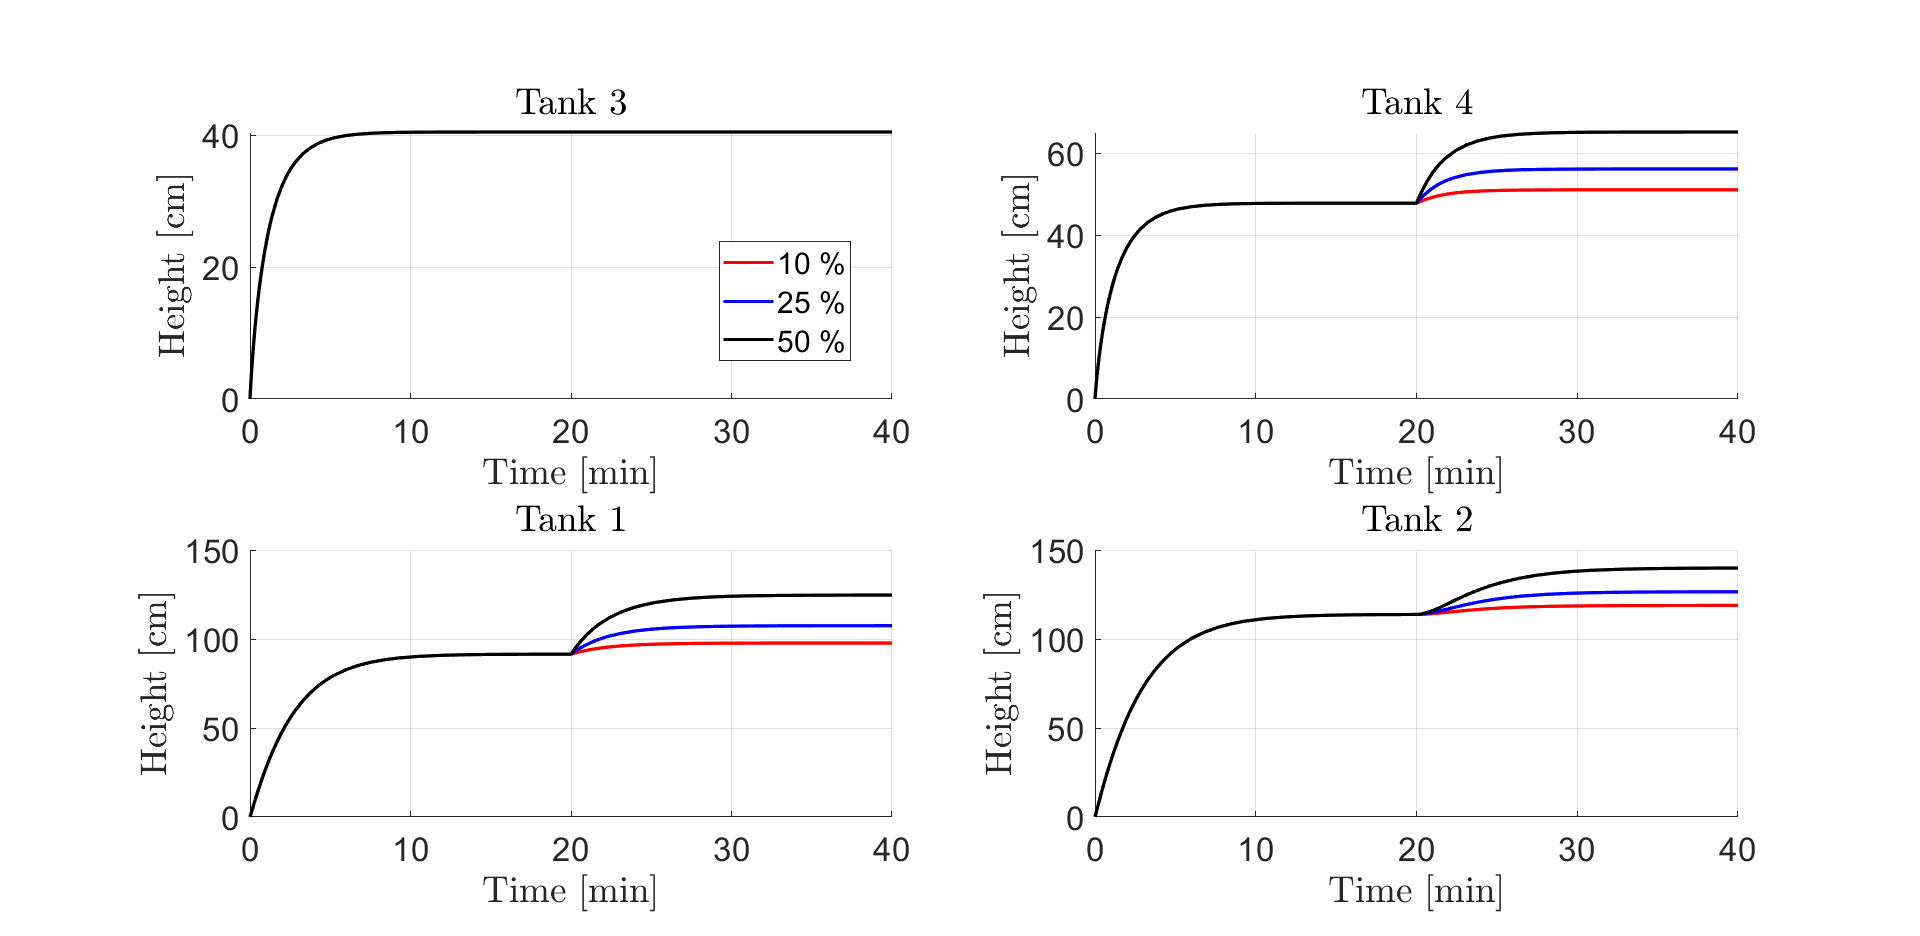
\includegraphics[width=1\textwidth]{Figures/Pr3.1_Det_Step u1.png}
    \caption{Step on $u_1$ - Deterministic model}
%    \label{fig:S}
\end{figure}
The different valve settings is seen in regards to the steady state response of the level in tank 1 and 2, where the water level is largest at tank 2, which is consistent with the valve setting $\gamma_1$ allows more water (compared to $\gamma_2$) going to tank 4 and thereby to tank 2.\\
It is seen that the step on $u_1$ do not affect tank 3 as expected, since this is only influenced by the disturbance and on $u_2$
\begin{figure}[H]
    \centering
    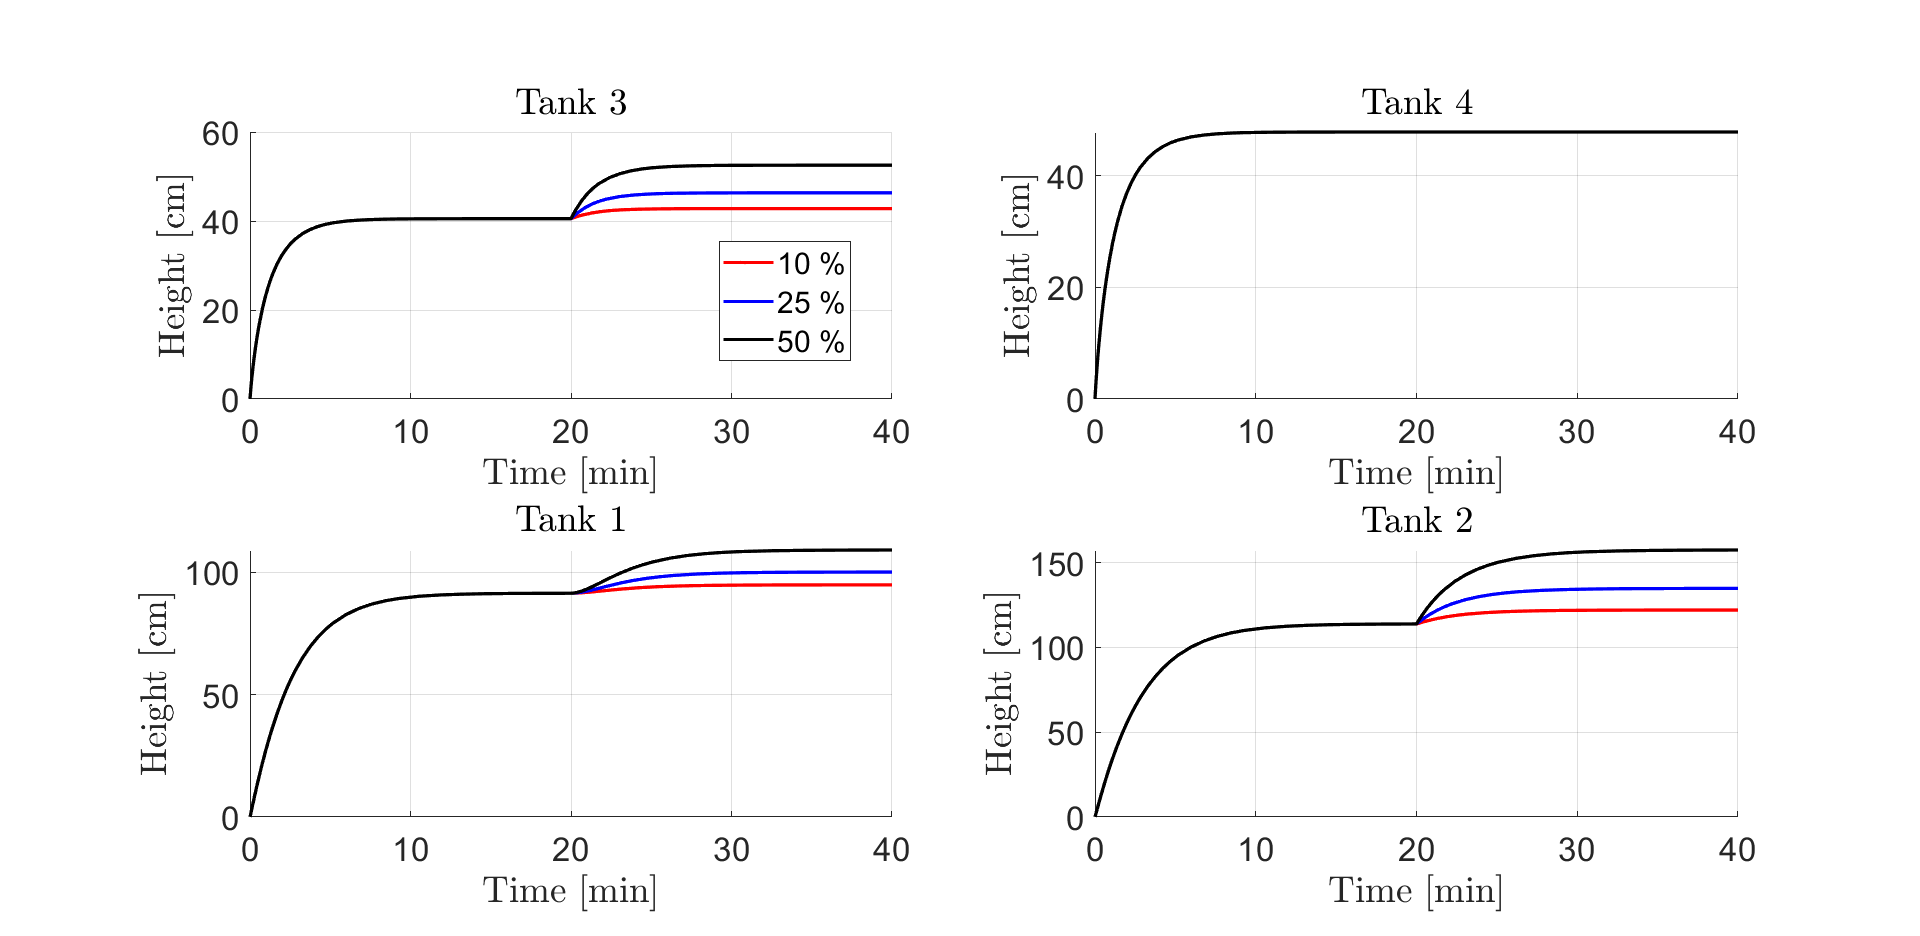
\includegraphics[width=1\textwidth]{Figures/Pr3.1_Det_Step u2.png}
    \caption{Step on $u_2$ - Deterministic model}
%    \label{fig:S}
\end{figure}
The behaviour of the system is, as expected, opposite of when input 1 is affected. 